%!TeX root=../thesisStructure.tex
% Chapter 1
\chapter{Introducción} % Chapter title
\label{ch:protocolo} 

En las próximas décadas, el acceso a agua potable se convertirá posiblemente en un reto para las futuras generaciones. La carencia de agua debido a las sequías de lluvia y procesos de potabilización o tratamiento deficientes 
tienen la etiqueta de convertirse en 2 de las principales causas de dicho problema \cite{ramadhan_smart_2020}.

La mayoría de los cuerpos de agua tales como ríos, lagos o arroyos, poseen ciertas
características que determinan su calidad. De la misma forma, dependiendo del uso o 
aplicación que tendrá un determinado volumen de agua, se tienen que cumplir características específicas \cite{bahita2021}. 
Por ejemplo, según \cite{aldhyani_water_2020} al agua usada para riego no debe ser demasiado salina ni
contener materiales tóxicos que pudiesen transferirse a las plantas o el suelo, 
dañando de esa manera el ecosistema en cuestión. Igualmente, el agua usada en procesos
industriales también requerirá cumplir estándares específicos dependiendo del
tipo de proceso, es decir, los requerimientos para agua usada en un proceso de producción
de alimentos serán diferentes a los requeridos para un proceso de generación en
una central hidroeléctrica.

Por otro lado, el crecimiento exponencial del área industrial ha provocado el decaimiento de la
calidad del agua en muchas regiones del mundo, llegando a niveles alarmantes e
inaceptables. Esto directamente tiene sus efectos de manera inmediata 
en el agua destinada para consumo humano \cite{akkoyunlu2012}. Según reportes de la ONU (Organización
de las Naciones Unidas), en los países en proceso de desarrollo se estima que el
80\% de las enfermedades son ocasionadas por el consumo de agua contaminada, y que
ocurren 15 millones de muertes al año relacionadas al mismo factor \cite{aldhyani_water_2020}.

En \cite{penaMurillo_Potabilizacion_Rural} entre los temas tratados se incluyen las causas que generan la contaminación del agua, mencionándose como la principal a la contaminación provocada por actividades industriales.
Menciona como los vertederos de desechos de los grandes centros industriales inyectan a los cuerpos de agua enormes cantidades de sustancias químicas y bioquímicas que imponen altas demandas sobre el oxígeno en cuerpos de 
agua con bajos niveles de oxígeno disuelto, así como alta demanda bioquímica y química de oxígeno, y alta concentración de sólidos disueltos, lo que genera entornos acuáticos extremadamente tóxicos y nocivos para la salud 
humana. Entre las sustancias presentes en desechos industriales que representan un riesgo elevado para la salud humana se encuentran por ejemplo los metales pesados, tales como arsénico, plomo, mercurio, cadmio y zinc.

En \cite{cantonEcuador} se toca el tema de los efectos ocasionados en la salud de la población por el uso de agua no potable. Se menciona que el uso de agua insalubre puede generar epidemias ocasionales de enfermedades bacterianas 
y virales dadas por agentes infecciosos transportados al ser humano, tales como cólera y poliomielitis. Menciona además como la presencia de metales pesados originarios de desechos agrícolas, industriales y actividad urbana, 
puede a largo plazo ser perjudicial a la salud humana siendo posible causa de surgimiento de enfermedades como cáncer, daño en órganos internos, alteraciones en el sistema nervioso e inmunológico. Referente específicamente 
a la actividad agrícola, el trabajo \cite{rio_Cunas} menciona estas actividades como un importante vertedero de nitrógeno, fósforo y plaguicidas en cuerpos de agua.

Para el ámbito tratado en este proyecto, la calidad del agua se define como el conjunto de parámetros
fisicoquímicos que determinan o son indicadores del nivel de contaminación de una muestra de agua \cite{zhang_characterization_2015}. Referente a esto, una parte fundamental respecto a la calidad del agua es acerca del tipo 
de aplicación, es decir, según la aplicación o uso que tendrá una determinada muestra de agua, es que se puede definir como adecuada o no la calidad del agua registrada. Un ejemplo simple sería el caso de agua potable y agua 
pura; el agua potable es para uso humano pero no es bebible, mientras que el agua pura tiene como propósito ser apta para beberse. Por lo tanto, en ambos casos se tienen estándares propios de calidad necesarios, sin embargo,
el agua pura conlleva mayores restricciones.

Los modelos matemáticos de IA (Inteligencia Artificial) están extendiendo continuamente sus 
posibilidades de aplicación, conforme dichos modelos son mejorados y optimizados, al mismo tiempo que las capacidades
de procesamiento de las computadoras crecen notablemente, dándonos la posibilidad de implementar algoritmos 
de aprendizaje automático y reconocimiento de patrones de una forma más sencilla.

Un conjunto de modelos de IA que han demostrado ser útiles para la determinación de la calidad del agua son los clasificadores. 
Estos algoritmos son estructuras matemáticas cuya finalidad consiste en predecir un valor o target (objetivo),
dado un conjunto de datos de entrada. Para el caso de análisis de calidad del agua es viable obtener datos de parámetros fisicoquímicos y biológicos de diferentes muestras de agua, con los cuales es posible optimizar un 
modelo de clasificación para realizar estimaciones del nivel de calidad del líquido \cite{barzegar_short-term_2020}.

Los trabajos de \cite{ramadhan_smart_2020} \cite{saetta_datamining_2021} \cite{mamun_smart_2019} se basan en la recolección de datos de diversas
variables, entre ellas ORP (Potencial de Oxidación y Reducción), conductividad,
pH (Potencial de Hidrógeno), concentración de nitratos, oxígeno disuelto, contenido 
de sodio, presencia de partículas sólidas y concentración de cloro. La metodología en estas investigaciones
se basa principalmente en el Internet de las Cosas para monitoreo en 
tiempo real mediante el uso de sensores en el lugar de interés, los cuales se
comunican con tarjetas de desarrollo basadas en microcontrolador.
Posteriormente, los datos recolectados se envían a un servidor Web para su 
procesamiento mediante técnicas estadísticas de regresión lineal o minería de datos.

El presente trabajo de investigación tiene como fin desarrollar modelos
de clasificadores entrenados con datos de variables 
fisicoquímicas del agua, los cuales serán recolectados de muestras correspondientes
a las fases de un proceso de potabilización. El objetivo del modelo de clasificación será realizar estimaciones de la calidad del agua para las muestras del proceso de potabilización usando información de los parámetros 
considerados para la optimización del clasificador.


%---------------------------------------------------------------------------------------------------------------------------------

\section{Revisión del estado del arte}

En esta sección se presenta la revisión de los diferentes trabajos analizados para tener un soporte teórico previo al desarrollo experimental del presente proyecto. Inicialmente se buscó información referente al tópico general 
de calidad del agua, para conocer sus definiciones y diferentes tratamientos o enfoques que puede tener este tópico. Posteriormente, la búsqueda de referencias teóricas se enfocó sobre los diferentes parámetros físicos, 
químicos y biológicos usados en los diversos procesos de monitoreo y control de calidad del agua, lo cual nos aporta soporte teórico sobre los parámetros conocidos previamente, así como otros parámetros que pudiesen ser 
incluidos en esta investigación. Finalmente, se realiza la búsqueda de trabajos de investigación similares a lo planteado para el presente proyecto, es decir, otras investigaciones enfocadas en análisis, estimación o control 
de la calidad del agua mediante el uso de modelos de IA o métodos estadísticos.

En el trabajo \cite{sanctuary_what_nodate} se describe la calidad del agua como 
sus condiciones, incluyendo los parámetros físicos, químicos y biológicos. Y estos 
parámetros se evalúan con la condición de si la muestra de agua es adecuada 
para un fin en específico, como podría ser consumo humano o agricultura. Se menciona 
que la calidad del agua se puede determinar con base en los valores de variables como
la concentración de oxígeno disuelto, concentración de bacterias, salinidad,
la turbidez, concentración de algas y presencia de partículas de metales pesados. De
igual forma, se establece que la determinación del nivel de la calidad del agua 
en una muestra determinada, debe realizarse de forma relativa conforme a la 
aplicación que tendrá dicha muestra.

El trabajo \cite{geetha_internet_2016} define el Monitoreo de la Calidad del Agua
como la recolección de información en diferentes lugares a intervalos regulares
de tiempo, con el objetivo de proveer con datos acerca de las condiciones actuales 
de los lugares estudiados. Establece que los principales objetivos del monitoreo 
de la calidad del agua incluyen la medición de parámetros críticos, tales como 
concentración microbiana y propiedades físicas y químicas, con el fin de hallar
cambios no deseados en los valores de los parámetros y proveer de advertencias 
acerca de que se ha identificado una situación de riesgo. Adicionalmente, el 
monitoreo en tiempo real permite la recolección de grandes volúmenes de datos, lo 
cual a su vez permite realizar medidas correctivas de manera más eficiente. 

En nuestro país México existen 2 normas regulatorias emitidas a través del Diario Oficial de la Federación del Gobierno de México como parte del conjunto de normas NOM (Norma Oficial Mexicana) que regulan un amplio rango 
de áreas en nuestro territorio. La primera norma a saber es la \textbf{NOM-127-SSA1-2021. Agua para uso y consumo humano. Límites permisibles de la calidad del agua}. Esta regulación es elaborada en conjunto con las Secretaría 
de Salud del gobierno mexicano y la Comisión Federal para la Protección contra Riesgos Sanitarios (COFEPRIS); en ella se trata como objetivo y campo de aplicación el establecimiento de los límites de calidad que debe cumplir 
el agua en México para uso y consumo humano. Además, para esta regulación se establece su observancia y cumplimiento obligatorio en el territorio nacional para los organismos responsables de los sistemas de abastecimiento 
de agua tanto públicos como privados \cite{nom-127-ssa1-2021}. En esta norma se define un proceso de potabilización como un conjunto de operaciones y procesos, físicos, químicos y biológicos, que se aplican al agua en los 
sistemas de abastecimiento de agua, con el fin de hacerla apta para el uso y consumo humano. Entre las restricciones incluidas en esta regulación se encuentran las siguientes, por ejemplo, que los sistemas de abastecimiento 
no deben deben como fuente a aguas residuales tratadas previamente; los límites permisibles para el parámetro de pH a la salida de un proceso de potabilización es en el rango de 6.5 a 8.5 en escala estándar; para el agua producto 
de un proceso de potabilización, el rango permisible para el parámetro de cloro residual es de 0.2mg/L a 1.5m/L \cite{nom-127-ssa1-2021}.  

La segunda norma regulatoria de relevancia en México viene siendo la \textbf{NOM-179-SSA1-2020. Agua para uso y consumo humano. Control de la calidad del agua distribuida por los sistemas de abastecimiento de agua}. En esta 
norma se establece que el agua destinada para uso y consumo humano, independientemente de la fuente de origen, superficial o subterráneo, debe de someterse a procesos de potabilzación con el propósito de evitar riesgos a 
la salud de la población y prevenir enfermedades infecciosas y parasitarias, así como las derivadas de la ingestión de sustancias tóxicas que pueda contener el agua. Esta norma define el agua para uso y consumo humano a 
toda aquella que no causa efectos nocivos a la salud y que no presenta propiedades objetables o contaminantes en concentraciones fuera de los límites permisibles y que no proviene de fuentes de aguas residuales tratadas.
Entre las restricciones señaladas en esta norma se encuentran las siguientes, por ejemplo, que todo proceso de potabilización debe contar con la documentación sobre su procedimiento de operación en la que se describa detalladamente 
la realización de cada una de las operaciones; tener la documentación de un programa de control analítico de la calidad del agua en el cual se señale los puntos de muestreo, parámetros de control y frecuencia de muestreo; 
para parámetros de control que rebasen los límites permisibles, se debe realizar el tratamiento correspondiente para su eliminación; se debe contar con un calendario para las acciones de mantenimiento preventivo así como 
llevar el registro de todas las operaciones preventivas y correctivas; efectuar inmediatamente la notificación a la COFEPRIS y a las instancias estatales de protección civil en caso de detección de emergencias sanitarias, 
en cuyo caso serán dichas instancias estatales y federales las encargadas de tomar decisiones sobre las acciones a llevar a cabo \cite{nom-179-ssa1-2020}.

En el trabajo \cite{rajib_rapid_2019} se hace una descripción del parámetro Potencial de Oxidación y Reducción (ORP), el cual es 
una medida de la tendencia de una sustancia para ganar electrones y ser reducida. Se 
establece que el ORP es energía potencial eléctrica almacenada en un líquido, y dicho potencial es útil para 
determinar las condiciones oxidativas o reductivas de la sustancia. Finalmente, se establece que la condición oxidativa 
de una sustancia se asocia con los valores positivos en milivolts (mV) de ORP, y la condición reductiva se 
asocia con los valores negativos.

El trabajo \cite{merida_cano_calidad_2020} realiza una investigación en la cual se presenta
la relación existente entre las propiedades bacteriológicas del agua y el Potencial de Oxidación y Reducción (ORP) en una planta potabilizadora. Para lo anterior, se llevó a cabo un monitoreo 
determinando los valores de ORP y coliformes fecales y totales en las unidades de filtración y en 
tanque de almacenamiento con agua desinfectada. Acorde a sus resultados, la presencia de coliformes fecales
y totales se dió con valores promedio de ORP de 250 mV, y la ausencia de estos se presentó con un ORP 
promedio de 760 mV.

En \cite{merida_cano_calidad_2020} se menciona que diversas investigaciones han demostrado que un valor de 
ORP en un rango de 650 mV a 700 mV, permite observar un decaimiento o disminución de bacterias, incluyendo
los casos como la bacteria \textit{E. Coli}, la cual muere en segundos al alcanzar valores de ORP en ese rango. Además,
se hace mención a que en el año de 1971, la Organización Mundial de la Salud (OMS) determinó que el ORP representa 
una alternativa altamente confiable para verificar la calidad sanitaria del agua, estableciendo que 
valores de ORP mayores a 650 mV indicarán la ausencia de concentraciones de microorganismos patógenos en el 
agua. Por lo tanto, los estándares de la OMS ya indican la relación existente entre el ORP y la calidad del agua, 
teniendo una desinfección casi instantánea al llegar a valores de ORP de 650 mV.

Los investigadores en \cite{merida_cano_calidad_2020} concluyen que para un proceso de potabilización
el ORP representará una medida de qué tan activos se encuentran los desinfectantes agregados durante el proceso,
mas no el nivel de concentración de los mismos. Señalan además que la 
utilización del ORP como un método alternativo para el control bacteriológico del agua en una planta potabilizadora es
viable, teniendo la ventaja de la existencia de equipo de instrumentación capaz de entregar datos en tiempo real.

En \cite{suslow_oxidation-reduction_2004} se analiza la variable ORP, destacando su importancia actual para el estudio
de la calidad del agua, señalando que dicha variable se ha convertido en un enfoque primario para la estandarización 
de otros parámetros usados en al análisis de calidad del agua. El autor indica la propiedad del agua al alcanzar valores 
en el rango de 650 mV y 700 mV para el ORP, como el potencial antimicrobiano del líquido es capaz de eliminar prácticamente en 
su totalidad a los organismos patógenos que pudieran estar presentes, teniendo tiempos menores a los 30s para lograr 
acabar con todas estas bacterias.

La investigación \cite{foladori_evolution_2018} se enfoca en la descripción y comparativa de diferentes técnicas de monitoreo de calidad del agua en un proceso de tratamiento de aguas residuales en la ciudad de Trento, Italia. 
Los autores hablan de que las técnicas tradicionales de análisis químico son esenciales para determinar las cargas de contaminantes eliminadas durante los procesos de tratamiento, pero este tipo de pruebas resultan 
costosas, consumen mucho tiempo y no se pueden implementar para monitoreo en tiempo real. Se menciona que para monitoreo en tiempo real de la 
calidad del agua se puede hacer uso de analizadores en línea para monitorear ciertos parámetros químicos, tales como la concentración de amonio, nitritos y fosfatos. 

El trabajo \cite{low_cost_Rao} propone la implementación de un sistema de monitoreo de bajo costo para calidad del agua en la ciudad de Melbourne en Australia. Habla de que los métodos convencionales que usualmente usan 
en dicha comunidad es monitoreo de calidad del agua de baja resolución dada por recolección de muestras en cuerpos de agua dulce, para su posterior análisis químico en laboratorio. Los autores indican que entre las desventajas 
de esta metodología se encuentran que la recolección de datos es irregular en tiempo y espacio, lo cual genera que eventos puntuales de contaminación no sean identificados. Por lo tanto, los investigadores proponen un sistema basado en la plataforma de hardware Arduino Mega para recolectar y procesar los datos de diferentes sensores
para un conjunto de parámetros, tales como temperatura, iluminación, pH, conductividad eléctrica, sólidos disueltos totales, salinidad, oxígeno disuelto y ORP. Con esta instrumentación se logró implementar un sistema 
de monitoreo continuo de las condiciones del agua, permitiendo así identificar nuevas fuentes de contaminación.

En \cite{Cambioclimatico} se realiza un estudio de la caracterización fisicoquímica del agua de lluvia captada en las instalaciones de la Academia Mexicana de Ciencias, con 
el fin de recolectar información sobre los sistemas de captación de agua de lluvia como alternativa al suministro de agua convencional. Se realizaron pruebas 
fisicoquímicas del agua de lluvia captada, dichas mediciones fueron sobre los parámetros de turbiedad, color aparente y verdadero, pH, sólidos disueltos, Carbono Orgánico 
Total y Demanda Química de Oxígeno. Los resultados obtenidos fueron comparados con la norma NOM-127-SSA1-2021, la cual establece a nivel nacional los límites máximos permisibles 
del agua potable. La comparación de los análisis contra la norma establecida arrojó que 5 de los parámetros se encuentran dentro del límite permisible y la variable turbiedad se 
encuentra por encima de los permitido. Lo anterior permite concluir que el agua de lluvia cuenta con la calidad suficiente para consumo humano, únicamente sería necesario la 
implementación de un sistema de filtrado de arena sílice que ayude a eliminar la materia en suspensión y así poder llevar el parámetro de turbiedad a valores adecuados.

El artículo \cite{conaguaManualPotabilización} publicado por la Comisión Nacional del Agua trata sobre los procesos de pretratamiento y tratamiento primario de aguas residuales.
En él, se abordan las características del proceso de pretratamiento y tratamiento primario, haciendo énfasis en la explicación de las diferentes etapas que conlleva, tales como 
el uso de rejas y rejillas para una primera etapa de filtración, posteriormente una segunda etapa de filtración mediante el uso de desarenadores. Como etapas siguientes se 
encuentran 2 procesos de sedimentación (primario y secundario), para finalmente llevar a cabo la etapa de cloración.  

En el trabajo \cite{paper01_MynorRomero} se profundiza sobre la etapa de cloración en los procesos de tratamiento de agua. Menciona que la adición de cloro en las etapas iniciales del proceso tiene 2 propósitos, desinfección y oxidación. Con estas dos propiedades se 
logra eliminar hierro, manganeso, sulfuros, amoniaco y otras sustancias reductoras. También se reducen sabores existentes antes de la cloración y la función que más interesa es la reducción del crecimiento de algas y otros      
microorganismos presentes en el agua. Esto se consigue añadiendo cloro hasta conseguir cloro residual libre en el agua. El cloro se puede adicionar en forma de cloro líquido, solución de hipoclorito de sodio o tabletas de 
hipoclorito de calcio.

El autor en \cite{paper01_MynorRomero} también trata el tema de los procesos de Coagulación-Floculación. Menciona que muchas impurezas se encuentran en el agua superficial como materia en suspensión y materia coloidal. Las    
especies coloidales incluyen arcilla, sílice, hierro, otros metales y sólidos orgánicos. La eliminación de una gran proporción de estas impurezas se lleva a cabo por sedimentación, basada en simple gravedad, pero algunas 
de estas impurezas son demasiado pequeñas para obtener un proceso de eliminación eficiente. La coagulación y floculación generan la rápida aglomeración de estas pequeñas impurezas, disminuyendo así el tiempo de sedimentación 
de las partículas. Para realizar este tipo de procesos se adicionan sales químicas en su mayoría cargadas positivamente (sales de aluminio, sales de hierro o polielectrolitos) que desplazan los iones negativos y reducen 
efectivamente el tamaño de carga eléctrica. Entre los floculantes más usados se tienen el sulfato de aluminio, polielectrolitos, cloruro férrico, sulfato ferroso y férrico.

El artículo \cite{paper02_TAR_Sevilla} trata sobre las características de un proceso de potabilización en la comunidad de Sevilla en España. El primer aspecto que trata esta publicación es el tema del proceso de oxidación 
que se lleva a cabo, mencionando sus 3 principales propósitos; el primero, la eliminación de sustancias disueltas en el agua, ya sea inorgánicas tales como ciertos minerales u orgánicas tales como ácidos de dicha naturaleza;
el segundo, eliminación de olores y sabores provocados por los compuestos orgánicos; el tercero, eliminación de gérmenes y agentes patógenos causantes de enfermedades. Entre los métodos de oxidación menciona 
4 casos; el primero, la aireación, que consiste en poner el agua en contacto con el aire, lo cual se puede lograr con turbinas o inyectores; el segundo, la adición del compuesto permanganato potásico el cual es muy 
efectivo en la oxidación de minerales; el tercero, adición de cloro y sus derivados, tales como gas cloro, hipoclorito. hipoclorito cálcico y dióxido de 
cloro; el cuarto, adición de ozono, el cual posee una alta capacidad oxidativa.

El trabajo \cite{paper02_TAR_Sevilla} profundiza además sobre los procesos de coagulación y floculación. Describen al proceso de coagulación como el encargado de desestabilizar la carga eléctrica exterior de las partículas 
coloidales, evitando la repulsión entre ellas y al mismo tiempo favoreciendo reacciones entre sí, generando la formación de coágulos o aglomeraciones de mayor densidad, lo cual facilita su sedimentación. Menciona 
que los coagulantes más utilizados son sulfato de aluminio, cloruro de aluminio, cloruro férrico y sulfato férrico. Respecto a la floculación, menciona que los 
agentes floculantes son sustancias con la facultad de captar los coágulos formados, logrando así generar masas de partículas contaminantes más voluminosas, lo que facilita la separación por sedimentación.

En \cite{evaluacionSubachoque} el autor realiza una descripción de parámetros fisicoquímicos de calidad del agua en el Rio Subachoque ubicado en Colombia. Habla del parámetro Sólidos Totales, el cual lo define como la totalidad
de materiales suspendidos o disueltos en el agua. Menciona que los cuerpos de agua con altas concentraciones de sólidos disueltos habitualmente se vuelven complejos de poder realizar adecuados procesos de potabilización

Ahora, para el tratamiento de los grandes volúmenes de datos que se recolectan, se 
han implementado diferentes métodos con diferentes conjuntos de parámetros.

El trabajo \cite{barzegar_short-term_2020} se centra en el análisis de los 
parámetros de Oxígeno Disuelto y la concentración de la sustancia Clorofila tipo A.
Se especifica que el parámetro de la concentración de Oxígeno Disuelto permite
conocer en una muestra de agua el equilibrio entre los procesos que producen
oxígeno y los procesos que requieren de él. Mientras que la sustancia Clorofila 
tipo A ayuda a realizar estimaciones de la concentración de algas.
El equipo que realizó esta investigación uso 2 técnicas del área de Deep Learning,
específicamente los modelos de Redes Neuronales Convolucionales (CNN) y Memoria
Larga a Corto Plazo (LSTM). El objetivo de las implementaciones de estos
algoritmos fue la predicción de los parámetros de Óxígeno Disuelto y Clorofila tipo 
A, haciendo uso de datos recolectados para otros parámetros, tales como pH, ORP,
temperatura y conductividad.

La investigación \cite{zhang_characterization_2015} se basa en el análisis de los
parámetros de ORP, conductividad, turbidez y concentración de Clorofila tipo A. En 
este caso, los investigadores realizaron un análisis estadístico de la varianza de 
los datos, usando el método ANOVA, para determinar si el nivel de la calidad del 
agua era influido por la profundidad a la cual se hacen las mediciones. Las 
conclusiones para este trabajo establecieron que el nivel de calidad de agua sí 
varía según el nivel de profundidad de donde se recolecten datos, ya que los 
parámetros estudiados presentaron variaciones conforme se analizaban datos 
correspondientes a diferentes profundidades.

El trabajo realizado en \cite{saetta_datamining_2021} presenta como objetivo 
la implementación de una plataforma de monitoreo de la calidad del agua, que incluya
la adquisición de datos y su almacenamiento, para posteriormente aplicar técnicas de
Minería de Datos y encontrar formas de mejorar la calidad del agua en la ciudad 
donde se realizó la investigación, usando las conclusiones que los algoritmos 
proporcionaban. Los parámetros analizados para este trabajo fueron temperatura, pH,
conductividad, ORP, Oxígeno Disuelto y concentración de cloro. 

La investigación \cite{hmoud_al-adhaileh_modelling_2021} tiene como objetivo la aplicación de los métodos Feed-Forward Neural Network (FFNN, Red Neuronal con retroalimentación) y 
K-nearest neighbors (KNN, K-vecinos más cercanos) para poder realizar clasificación de calidad del agua. En este trabajo se reunieron datos de 8 parámetros, 
oxígeno disuelto, pH, conductividad, demanda biológica de oxígeno, concentración de nitratos, coliformes fecales, temperatura y coliformes totales. Los resultados que obtuvieron 
en esta investigación alcanzaron el 100\% de porcentaje de aciertos para Clasificación de Calidad del Agua (WQC, Water Quality Classification). 

La investigación \cite{waterQuality_Supervised_ML} trata sobre la aplicación de un conjunto de algoritmos de Machine Learning con aprendizaje supervisado para análisis de calidad del agua en una cuenca acuática en el país 
de Pakistán. Sus objetivos fueron la estimación del índice de calidad del agua (\textit{Water Quality Index}, \textbf{WQI}), así como la clasificación de calidad del agua (\textit{Water Quality Class}, \textbf{WQC}); los 
parámetros utilizados para el entrenamiento de los modelos fueron pH, turbidez, temperatura y sólidos disueltos totales. Para la estimación del WQI se usaron los algoritmos de regresión lineal, regresión polinomial, árboles 
aleatorios (\textit{Random Forest}), gradient boosting, máquinas de soporte vectorial (\textit{Support Vector Machine}, \textbf{SVM}), regresión Ridge, regresión Lasso y regresión de Red Elástica; de este conjunto de algoritmos,
los modelos de gradient boosting con tasa de aprendizaje de 0.1 y la regresión polinomial de grado 2 tuvieron los mejores resultados, con errores absolutos medios de 1.9642 y 2.7273, respectivamente. Para el caso del cálculo 
de la WQC, se probaron los modelos Multi-Layer Perceptron (\textit{Perceptrón Multicapa}), clasificador Gaussiano Naive Bayes, regresión logística, descenso por gradiente estocástico, árboles de decisión, máquinas de soporte 
vectorial, clasificador Bagging y clasificador gradient boosting; los 2 modelos que obtuvieron mejor exactitud en las pruebas ejecutadas fueron MLP y regresión logística con valores de exactitud de 0.8507 y 0.8401, respectivamente.  

Los trabajos revisados en esta sección proporcionan el panorama existente sobre el tópico tratado en nuestro proyecto. Primeramente, las investigaciones enfocadas a definiciones básicas nos ayudan a comprender el concepto 
de calidad del agua y su posible impacto en otros entornos. Posteriormente, los trabajos enfocados a análisis y descripción de parámetros de calidad del agua, nos ayudan a conocer el amplio conjunto de variables específicas o que 
generan evidencia confiable para los estudios enfocados a cuidado y tratamiento del agua. Finalmente, las investigaciones sobre técnicas de IA para análisis de calidad del agua nos proporcionan información sobre los modelos 
de IA que ya han sido usados para este tipo de aplicación, y de esta forma conocer qué algoritmos podrían ser los más fiables para el proceso de potabilización tratado en este proyecto. 

\section{Planteamiento del problema} \label{sec:SolProp}

El proceso de potabilización llevado a cabo por parte de la oficina municipal del OOAPAS
implica la toma continua de muestras a lo largo de las diferentes etapas que lo componen,
además de que continuamente se reciben muestras tomadas de diferentes puntos de la ciudad.
El laboratorio de calidad del agua del OOAPAS se encarga de realizar análisis químicos y biológicos
para corroborar que su calidad sea acorde con los requisitos establecidos, y en caso de encontrar en
sus mediciones valores no deseados para los parámetros en estudio, llevar a cabo medidas correctivas 
y preventivas. 

El presente trabajo se enfoca en las estimaciones de los niveles de calidad del agua para el proceso de potabilización, mediante una metodología basada en el uso de instrumentación eléctrónica para la recolección de datos 
de parámetros del proceso de tratamiento. Estos datos serán posteriormente procesados con el uso de herramientas estadísticas de correlación para determinar las variables representativas del proceso. Finalmente, con estos
parámetros representativos se optimizará un modelo de clasificación basado en IA encargado de realizar las estimaciones de calidad del agua.

\section{Objetivos}

\subsection{Objetivo general}

%Determinar los parámetros fisicoquímicos más importantes en un proceso de
%potabilización, y encontrar cómo se relacionan estos parámetros con las variaciones
%en el nivel de calidad del agua, para poder desarrollar un clasificador basado 
%en Inteligencia Artificial que pueda determinar en una 
%muestra de agua si sus condiciones permiten catalogarla como agua potable.

Analizar y determinar los parámetros de calidad del agua más importantes en el proceso de potabilización estudiado, así como también estudiar su grado de correlación, con el objetivo de implementar un modelo de clasificación 
basado en inteligencia artificial para realizar estimaciones de calidad del agua para el mismo proceso de tratamiento. 
 

\subsection{Objetivos particulares}
\begin{itemize} 
	\item Identificar las fases de un proceso de potabilización.
	\item Obtener datos de los parámetros ORP, oxígeno disuelto y cloro residual, con lo cuales se pueda generar una caracterización del proceso de potabilización.
	\item Determinar el grado de correlación entre los 3 parámetros analizados.
	\item Definir un modelo de clasificación basado en Inteligencia 
	Artificial para estimaciones de calidad del agua.
	\item Generar diversas pruebas de entrenamiento y validación del modelo de IA elegido.
	\item Determinar el nivel de desempeño del modelo elegido para la base de datos generada.
\end{itemize}
%****************************************************************

\section{Hipótesis}

El estado del arte indica que el ORP puede considerarse el parámetro más significativo
para conocer la calidad del agua, sin embargo, en este proyecto se plantea el 
escenario de agregar parámetros adicionales y estudiar los efectos que esto
tendría. Es decir, investigar si más variables en consideración generan 
la optimización del proceso de determinar la calidad del agua, o su inclusión
resulta innecesaria.

Por lo tanto, el planteamiento para este trabajo es analizar 3 parámetros en un proceso de potabilización e implementar un algortimo de clasificación de calidad del agua que pueda ofrecer mayor nivel de certeza en sus 
estimaciones.


\section{Metodología}

Las actividades a realizar se especifican a continuación en el orden correspondiente
en que se realizarán.
\begin{itemize}
	\item Obtención de estándares teóricos de los 3 parámetros elegidos. Inicialmente,
	será necesario conocer el rango de valores que pueden tener las variables que se
	van a usar como datos para el modelo de Inteligencia 
	Artificial. Dentro del proceso de potabilización monitoreado se tendrá
	que conocer el rango de valores teóricos que pueden adoptar los parámetros 
	considerados, con el fin de tener la referencia para cuando sea
	el momento de realizar las mediciones, poder hacer una comparación entre lo 
	medido y lo teórico, y determinar, en caso de que los valores de los datos estén 
	fuera de los rangos teóricos, cuál es la causa de que las mediciones sean 
	diferentes.
	\item Medición de los parámetros. Se tendrá que asistir a la institución del 
	OOAPAS (Organismo Operador de Agua Potable, Alcantarillado y Saneamiento del 
	Municipio de Morelia), que es donde se llevan a cabo los procesos de potabilización
	y se nos permitirá el acceso para obtener los datos necesarios para el trabajo de
	investigación. El proceso de medición se llevará a cabo usando el equipo de 
	instrumentación WiFi Pool Kit, del fabricante Atlas Scientific. 
	Este equipo de medición cuenta con la posibilidad de conectar sondas de medición para las variables medidas, además de contar con circuitos para acondicionamiento de señal y un microcontrolador ESP32 para lectura y 
	almacenamiento de datos en una computadora externa. 
	\item Preprocesamiento de los datos. Generar un análisis de estadística descriptiva y correlación para conocer el comportamiento de los parámetros durante las diferentes fases de potabilización.
	\item Definición de un algoritmo de clasificación. Determinar qué modelo de clasificación basado en IA será utilizado para la base de datos generada. 
	\item Pruebas de entrenamiento y validación del modelo de clasificación. Para la base de datos generada a partir de la toma de muestras, elegir aleatoriamente una porción mayoritaria de dicho conjunto de información 
	para generar el entrenamiento del modelo de clasificación y sus respectivas pruebas de validación con el porcentaje de datos restantes.
\end{itemize}

En la \autoref{fig:figura1200_1} se muestra un esquema de la primera parte para el método planteado.

%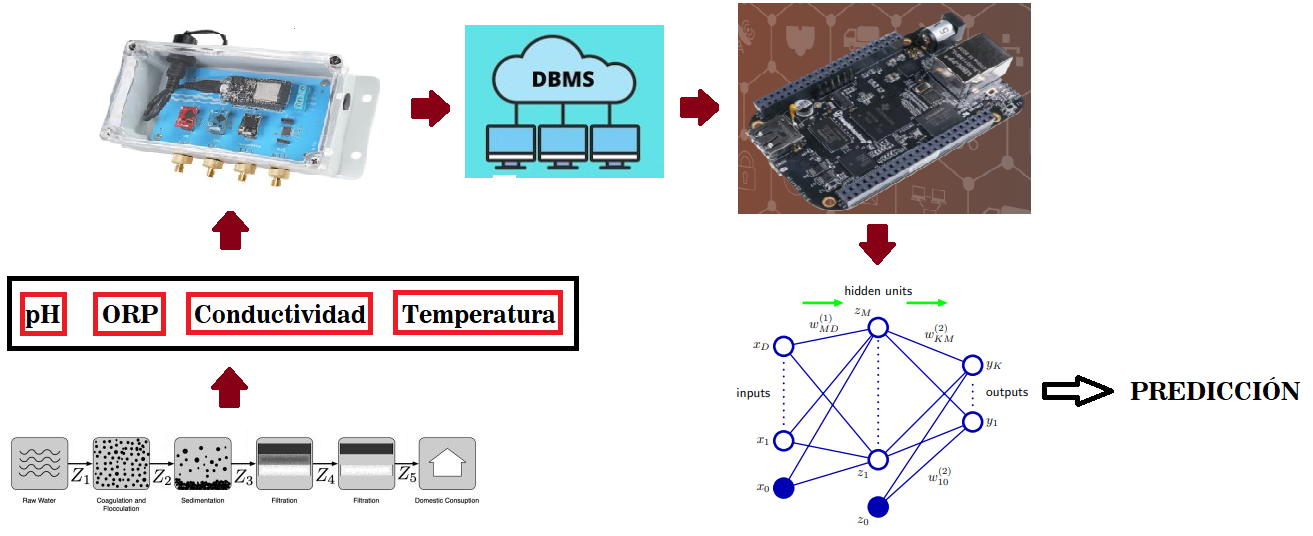
\includegraphics[scale=0.5]{figuraMetodología.png}[\centering]

%\begin{figure}[h]
	%\centering
	%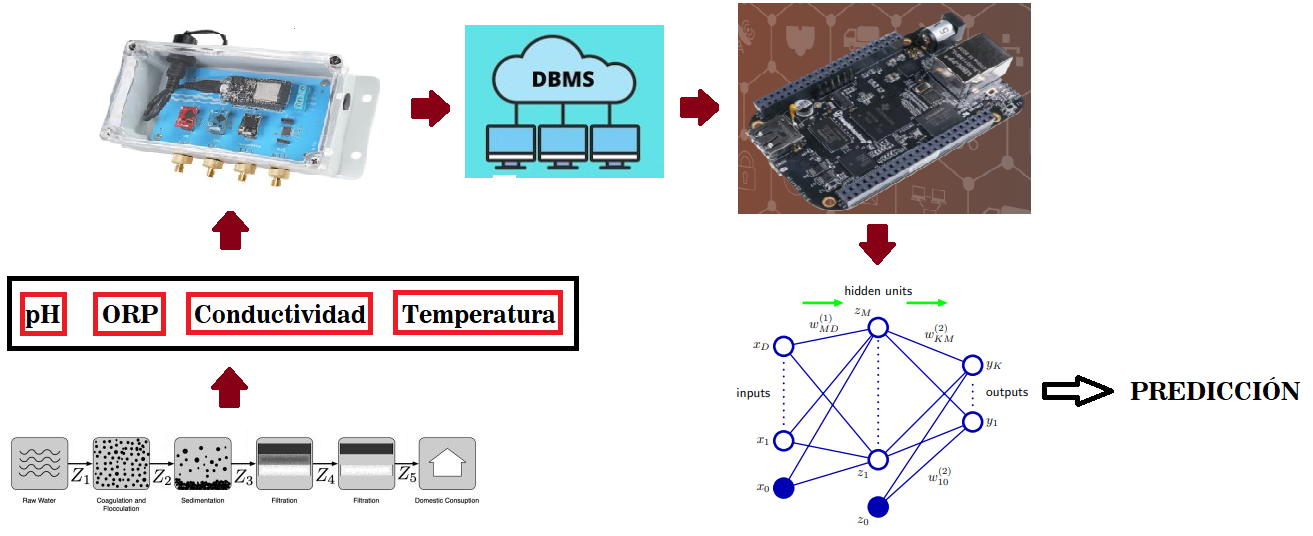
\includegraphics[scale=0.46]{figuraMetodología.png}
	%\caption{Función logística o sigmoide}
	%\label{fig:figura3_40}
%\end{figure}

%\clearpage

%\tikzstyle{startstop} = [rectangle, rounded corners, 
						%minimum width=3cm, 
						%minimum height=1cm,
						%text centered, 
						%draw=black, 
						%fill=red!30]

%\tikzstyle{io} = [trapezium, 
				  %trapezium stretches=true, % A later addition
				  %trapezium left angle=70, 
				  %trapezium right angle=110, 
				  %minimum width=3cm, 
				  %minimum height=1cm, text centered, 
				  %draw=black, fill=blue!30]

%\tikzstyle{process} = [rectangle, 
					   %minimum width=3cm, 
					   %minimum height=1cm, 
					   %text centered, 
					   %text width=3cm, 
					   %draw=black, 
					   %fill=orange!30]

%\tikzstyle{decision} = [diamond, 
						%minimum width=3cm, 
						%minimum height=1cm, 
						%text centered, 
						%draw=black, 
						%fill=green!30]
%\tikzstyle{arrow} = [thick,->,>=stealth]

%\begin{center}
%\begin{tikzpicture}[node distance=2cm]

	%\centering

	%\node (start) [startstop] {Etapas del Proceso de Potabilización};
	%\node (in1) [startstop, below of=start,yshift=-0.8cm] {pH	ORP		Conductividad		Temperatura};
	%\node (pro1) [startstop, below of=in1,yshift=-0.8cm] {Equipo WiFi Pool Kit};
	%\node (dec1) [startstop, below of=pro1, yshift=-0.8cm] {DBMS};

	%\node (pro2a) [startstop, below of=dec1, yshift=-0.8cm] {Tarjeta de desarrollo BeagleBone Black};
	
	%\node (pro2b) [process, right of=dec1, xshift=2cm] {Process 2b};
	%\node (out1) [startstop, below of=pro2a,yshift=-0.8cm] {Red Neuronal Artificial};
	%\node (stop) [startstop, below of=out1,yshift=-0.8cm] {Estimación de Calidad del Agua para una muestra};

	%\draw [arrow] (start) -- (in1);
	%\draw [arrow] (in1) -- (pro1);
	%\draw [arrow] (pro1) -- (dec1);
	%\draw [arrow] (dec1) -- node[anchor=east] {yes} (pro2a);
	%\draw [arrow] (dec1) -- node[anchor=south] {no} (pro2b);
	%\draw [arrow] (pro2b) |- (pro1);
	%\draw [arrow] (pro2a) -- (out1);
	%\draw [arrow] (out1) -- (stop);
														   
%\end{tikzpicture}
%\end{center}

%\clearpage

\begin{figure}[h]
	\centering
	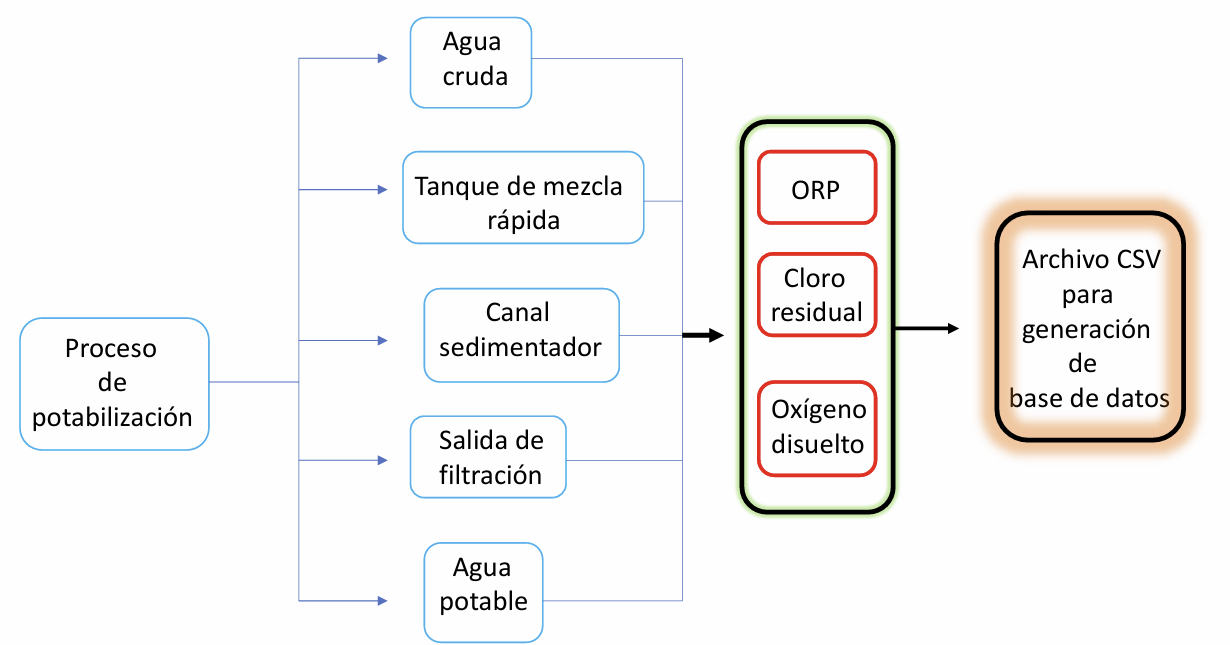
\includegraphics[scale=0.75]{imgss217.png}
	\caption{Método para generación de base de datos}
	\label{fig:figura1200_1}
\end{figure}

En el proceso de potabilización se han elegido 5 puntos específicos en los cuales se realizará la toma de muestras. Los puntos de muestreo en el proceso serán las fases de agua cruda, tanque de mezclado rápido, canal sedimentador,
la salida de filtración y finalmente el agua potable, que es el producto final del proceso de tratamiento.

Lo que se busca es lograr una caracterización del proceso mediante parámetros específicos. Por lo tanto, para cada muestra correspondiente a cada fase es necesario realizar la medición puntual o continua de los 3 parámetros 
considerados, que en este caso serán ORP, cloro residual y oxígeno disuelto. Cada vez que se realice una toma de muestras, el conjunto de mediciones registradas debe etiquetarse según la fase del proceso que corresponda, y 
gradualmente ir formando una base de datos más amplia.

En la \autoref{fig:figura1200_47} se muestra un esquema de la segunda parte para el método planteado.

\clearpage

\begin{figure}[h]
	\centering
	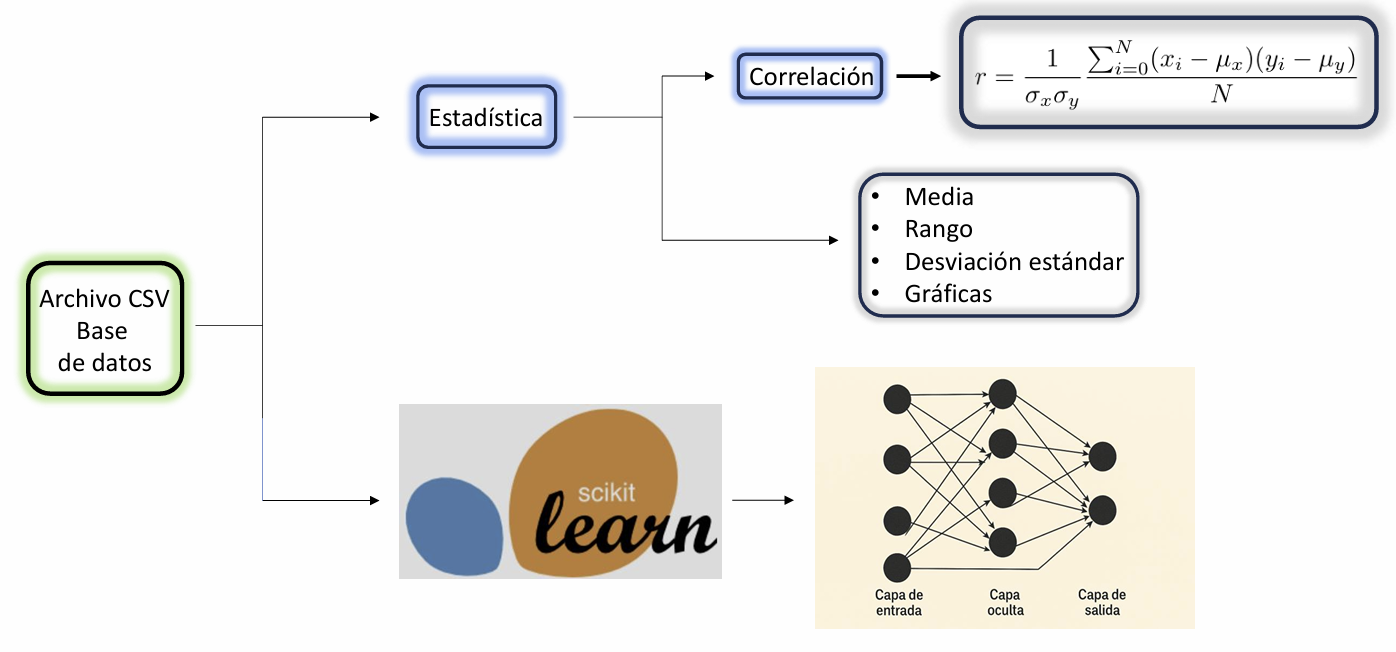
\includegraphics[scale=0.65]{imgss218.png}
	\caption{Método para tratamiento de la información}
	\label{fig:figura1200_47}
\end{figure}

Con la base de datos generada primero se realiza el análisis mediante herramientas estadísticas para conocer el comportamiento de cada parámetro medido. Se obtienen coeficientes de correlación lineal entre los 3 parámetros,
además de obtener métricas descriptivas y gráficas de los parámetros para las diferentes etapas del proceso de potabilización.

La base de datos recolectada igualmente servirá para optimizar el modelo de clasificación de calidad del agua. El conjunto de datos deberá particionarse aleatoriamente para generar grupos para entrenamiento y validación, y 
con ellos generar las pruebas necesarias hasta encontrar la mejor o mejores optimizaciones.

\clearpage

\section{Conclusiones}

En este capítulo se presenta la revisión del estado del arte en el cual se hace la exposición de trabajos teóricos acerca de los conceptos y definiciones relacionadas con la calidad del agua y los diferentes parámetros utilizados 
para su análisis. Adicionalmente, se incluyen investigaciones aplicadas en las cuales se hace uso de técnicas estadísticas y de inteligencia artificial para análisis de calidad, y dichos trabajos se pueden tomar como guía o 
referencia para el presente proyecto y así determinar que técnicas o modelos podrían adaptarse mejor a lo que nosotros realizamos.

Posteriormente, se exponen tanto los objetivos general y partículares para el proyecto con los cuales se define el propósito y alcance que se plantea para esta investigación, de acuerdo al proceso que va a estudiarse y los 
recursos con los que se trabajará. 

Finalmente, se expone el procedimiento o metodología general a seguir para lograr el alcance de los objetivos previamente establecidos. Se detalla que nuestra investigación inicia desde el conocer las características del 
proceso que se va a estar estudiando, sus diferentes parámetros y cómo se estarán midiendo para almacenar los datos monitoreados. Lo anterior con el fin de generar una base de datos que pueda caracterizar el proceso de 
potabilización y posteriormente servir para realizar estimaciones de calidad del agua mediante un modelo basado en inteligencia artificial.

\clearpage
